\documentclass[a4paper,10pt]{article}
\usepackage[paper=a4paper, left=1.5cm, right=1.5cm, bottom=2.0cm, top=1.6cm]{geometry}
\usepackage[utf8]{inputenc}
\usepackage[spanish]{babel}
\usepackage{color}
\usepackage{amsthm}
\usepackage[colorlinks=true, linkcolor=blue]{hyperref}

\usepackage{verbatim}
\usepackage{caratula1}
\usepackage{algorithm}
\usepackage{algpseudocode}
\usepackage{verbatim}
\usepackage{amsfonts}
\usepackage{amsmath}
\usepackage{graphicx}
%\usepackage{epstopdf}
\usepackage{ifpdf}
\usepackage{multicol}
\usepackage{caption}
\usepackage{subcaption}
%\usepackage{subfig}


\begin{document}
%Datos para la caratula
\materia{Teoría de las Comunicaciones}

\titulo{Trabajo Pr\'actico 1}

\subtitulo{Wiretapping}

%\grupo{Grupo ?}

\integrante{Dabbah, Juli\'an}{15/09}{djulius@gmail.com}
\integrante{Fern\'andez Abrevaya, Victoria}{710/10}{vabrevaya@gmail.com}
\integrante{Gonz\'alez, Sergio}{723/10}{sergiogonza90@gmail.com}

\maketitle
\tableofcontents
\newpage
  


\begin{abstract}
\textbf{Resumen:} 

\textbf{Palabras clave:} ARP, Teoría de la Información, Entropía, Scapy, Nivel de Enlace.
\end{abstract}

$\\$
\section{Introducci\'on}

El presente trabajo pr\'actico consiste en analizar las rutas que siguen los paquetes IPs al viajar largas distancias. Para ello implementaremos 2 herramientas basadas en el protocolo ICMP:
Ping y Traceroute.

El protocolo ICMP (Internet Control Message Protocol) suele utilizarse como un protocolo de control entre y notificacion de errores en el envio de paquetes IP, por lo que corre debajo de este mismo. Las herramientas Ping y Traceroute que se encuentran en los Sistemas Operativos mas utilizados utilizan este mismo protocolo.

Existen muchos tipos de paquetes ICMP que pueden mandarse, pero nosotros para la implementacion de las herramientas solo nos focalizaremos en 3:

\begin{itemize}
 \item Echo-Request
 \item Echo-Reply
 \item Time Exceeded
\end{itemize}

Cuando un host A quiere saber si un host B esta disponible, lo que hace es mandar un paquete ICMP (sobre uno IP) de tipo {\bf Echo-Request}. Si el servidor B esta disponible efectivamente, le envia al host un paquete ICMP de tipo {\bf Echo-Reply}.

Existe una propiedad de los paquetes ICMP denominada {\bf Time To Live} (o TTL) el cual indica el numero maximo de {\bf hops} que puede realizar el mismo. Cuando un router resive un paquete de tipo Echo-Request el cual tiene como TTL = 0, este manda un paquete ICMP de tipo {\bf Time Exceeded} al servidor origen Esto por ejemplo se puede utilizar para aproximar una ruta posible que sigue un paquete, enviando paquetse de tipo Echo-Request aumentando linealmente el TTL, y viendo que IPs fuente son las que nos mandan las respuestas de Time Exceeded, hasta que se recibe un Echo-Reply.

En base a este algoritmo se implementara la herramienta {\bf Traceroute}. Luego se utilizaran tanto estas herramientas como las ya implementadas en sistemas Unix para realizar mediciones y analisis en base a las rutas y los enlaces transoceanicos que se encuentren.

Para determinar si un enlace es Transoceanico lo que se hara sera es utilizar herramientas como las que se encuentran en \url{http://www.geoiptool.com/es/} o \url{http://geoip.flagfox.net/} Para poder localicar el punto geografico de un router mediante su IP publica.

%% ACA ME FALTA UN TOQUE, COMITIE PORQUE ME FUI A COMER :P

$\\$	
\section{M\'etodos}

% LES COPIO LO QUE TENGO ANOTADO EN EL CUADERNO:
% Hablar de entropia (como la vamos a tomar, como vamos a sniffear. Tambien puede ponerse un pseudocodigo, o una explicacion del codigo

\subsection{Primera Consigna: Implementaci\'on de un cliente ARP}
El primer paso consiste en implementar un cliente ARP, definiendo una funci\'on que, dada una direcci\'on IP, realice un pedido por la direcci\'on f\'isica asociada y, en caso de que reciba respuesta, la muestre. *** ESTO ES LO QUE HACEMOS??

\subsection{Segunda Consigna: Capturando tr\'afico}

\subsection{Tercera Consigna: Gr\'aficos y An\'alisis}

% Aca supongo que vamos a explicar que vamos a graficar, y en la proxima seccion ponemos los graficos que nos hayan dado.
$\\$	
\section{Resultados}

% LES COPIO LO QUE TENIA EN EL CUADERNO:
% 	Delays en distintos momentos del dia? 
%	Se congestionan los enlaces en horas pico? (ver cuales son las horas pico en cada pais del enlace). 
%	Se utilizan los enlaces si voy a otras paginas cercanas a las que probamos? 
%	Cambian las rutas que se toman a una misma pagina? 
%	Ver tiempos de encolamiento (hacer algun tipo de analisis sobre esto supongo)

%Los datos de los siguientes graficos se midieron utilizando el Traceroute implementado por nosotros. El metodo de medicion fue el siguiente:
Utilizando el \texttt{traceroute} implementado por nosotros, y las herramientas de localizaci\'on mencionadas, observamos los siguientes enlaces transoce\'anicos:

\begin{itemize}
 \item Enlace 1: Entre Estados Unidos (Florida seg\'un \emph{IP2Location}, Colorado seg\'un \emph{IPLigence}), e Inglaterra (seg\'un \emph{IP2Location}), que detectamos rastreando la ruta hacia \url{www.helsinki.fi} (IP: 128.214.222.4, Finlandia).
 \item Enlace 2: Entre Estados Unidos, Colorado (seg\'un \emph{IPligence}) y Alemania (seg\'un \emph{IPligence}), detectado en el camino a \url{www.ox.ac.uk} (IP: 163.1.60.42, Reino Unido).
 \item Enlace 3: Entre Estados Unidos, Colorado (seg\'un \emph{IPligence}) y Zurich, Suiza (seg\'un todas las herramientas consultadas), detectado rastreando la ruta hacia \url{web.up.ac.za} (IP: 137.215.78.74, Sud\'africa).
\end{itemize}

Estos enlaces se corresponden con las siguientes IPs:

\begin{itemize}
 \item Enlace 1:\\
    IP en Am\'erica (EEUU): 67.17.106.162\\
    IP en Europa (Reino Unido): 213.155.137.26
  \item Enlace 2:\\
    IP en Am\'erica (EEUU): 67.16.139.18\\
    IP en Europa (Alemania): 141.136.107.37
  \item Enlace 3:\\
    IP en Am\'erica (EEUU): 146.82.32.154\\
    IP en Europa (Suiza): 77.109.134.50
\end{itemize}


En las figuras \ref{fig:mapa_fin}, \ref{fig:mapa_ing} y \ref{fig:mapa_sud} se muestra una localizacion aproximada de los enlaces transoceánicos utilizados.\\

\begin{figure}[H]
  \centering
    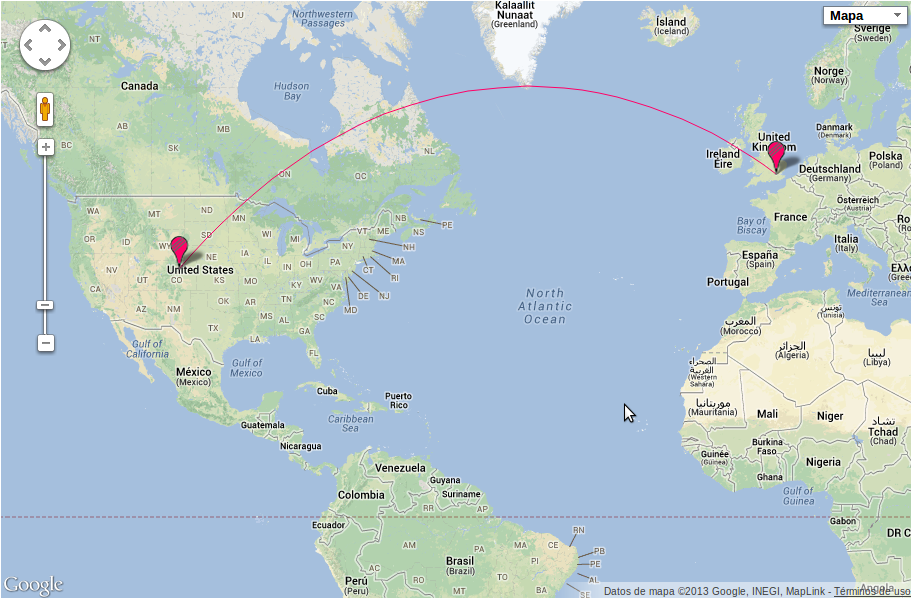
\includegraphics[width=0.9\textwidth]{imgs/finlandia_enlace_1.png}
    \caption{Mapa con la ubicación aproximada del enlace tomado hacia el host \url{www.helsinki.fi} (Finlandia)}
    \label{fig:mapa_fin}
\end{figure}    

\begin{figure}[H]
  \centering
    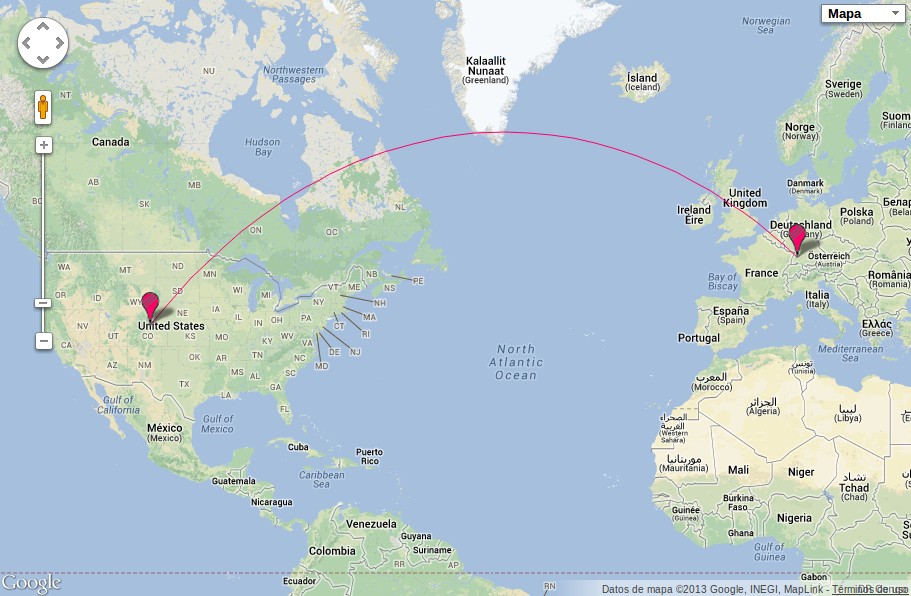
\includegraphics[width=0.9\textwidth]{imgs/inglaterra_enlace_1.png}
    \caption{Mapa con la ubicación aproximada del enlace tomado hacia el host \url{www.ox.ac.uk} (Reino Unido)}
    \label{fig:mapa_ing}
\end{figure}

\begin{figure}[H]
  \centering
    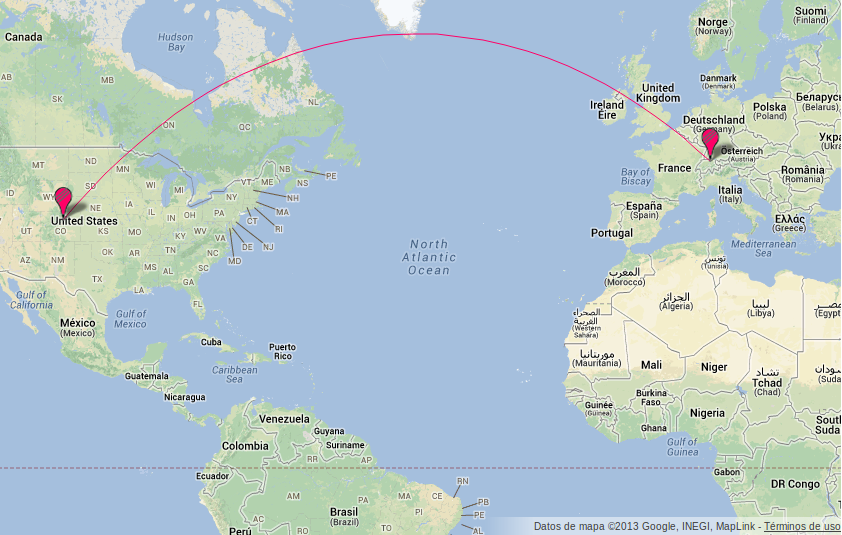
\includegraphics[width=0.9\textwidth]{imgs/sudafrica_enlace_1.png}
    \caption{Mapa con la ubicación aproximada del enlace tomado hacia el host \url{web.up.ac.za} (Sud\'africa)}
    \label{fig:mapa_sud}
\end{figure}

Las figuras muestran claramente que los enlaces encontrados son aproximados, ya que recorren una distancia por tierra que no esta siendo considerada por el \texttt{traceroute}. Es muy probable que en el camino entre los enlaces encontrados existan varios routers, lo cual no se est\'a teniendo en cuenta al considerarlo como una única conexión entre continentes.\\

Sabiendo la ubicaci\'on de cada extremo del enlace pudimos calcular su distancia, y en base a eso el RTT mínimo. Dado que los paquetes son pequeños despreciamos el tiempo de transmisión. Los datos obtenidos fueron los siguientes:

% TABLA
\begin{center}
\begin{tabular}{l l l  l}
  \label{tabla1}
 \textbf{Host Destino} & \textbf{Enlace} & \textbf{Distancia} & \textbf{RTT mínimo} \\
 \url{www.helsinki.fi} (Finlandia) & EE.UU - Inglaterra & 7543.656 km & 75.44ms\\
 \url{www.ox.ac.uk} (Reino Unido) & EE.UUU - Alemania & 8247.572 km & 82.47ms \\
 \url{web.up.ac.za} (Sud\'africa) & EE.UU - Suiza & 8319.832 km & 83.19ms \\
\end{tabular}
\end{center}

Tanto en el caso del host de Inglaterra como el de Finlandia, la ruta obtenida por nuestro \texttt{traceroute} no varió en ningún momento del día: los ips recibidos como parte de la ruta fueron siempre los mismos. En el caso de Sudáfrica sí se observaron diferencias, pero esas diferencias fueron de ips y no de ubicación (es decir, la ruta general seguida fue siempre la misma, si bien los routers particulares de cada lugar podían variar).\\

Las figuras \ref{fig:ruta_fin}, \ref{fig:ruta_ing} y \ref{fig:ruta_sud} muestran algunos de los nodos dentro de la ruta completa encontrada por el \texttt{traceroute}. Sólo se muestra la ubicación de una ip por cada país que recorrió el paquete.

\begin{figure}[H]
  \centering
    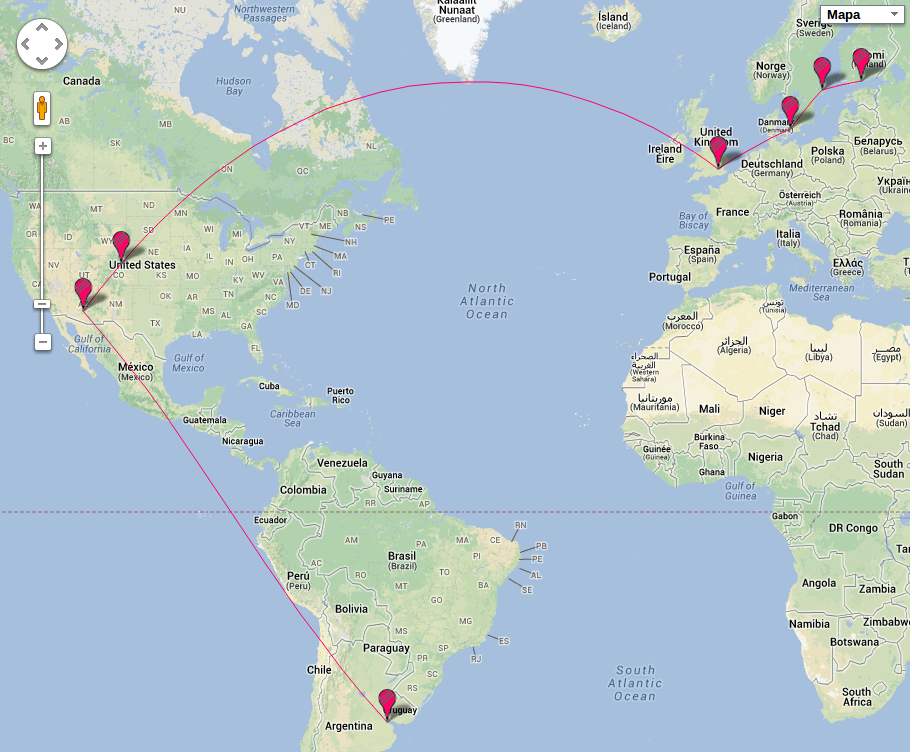
\includegraphics[width=0.9\textwidth]{imgs/finlandia_ruta_1.png}
    \caption{Mapa con la ruta aproximada hacia el host \url{www.helsinki.fi} (Finlandia)}
    \label{fig:ruta_fin}
\end{figure}    

\begin{figure}[H]
  \centering
    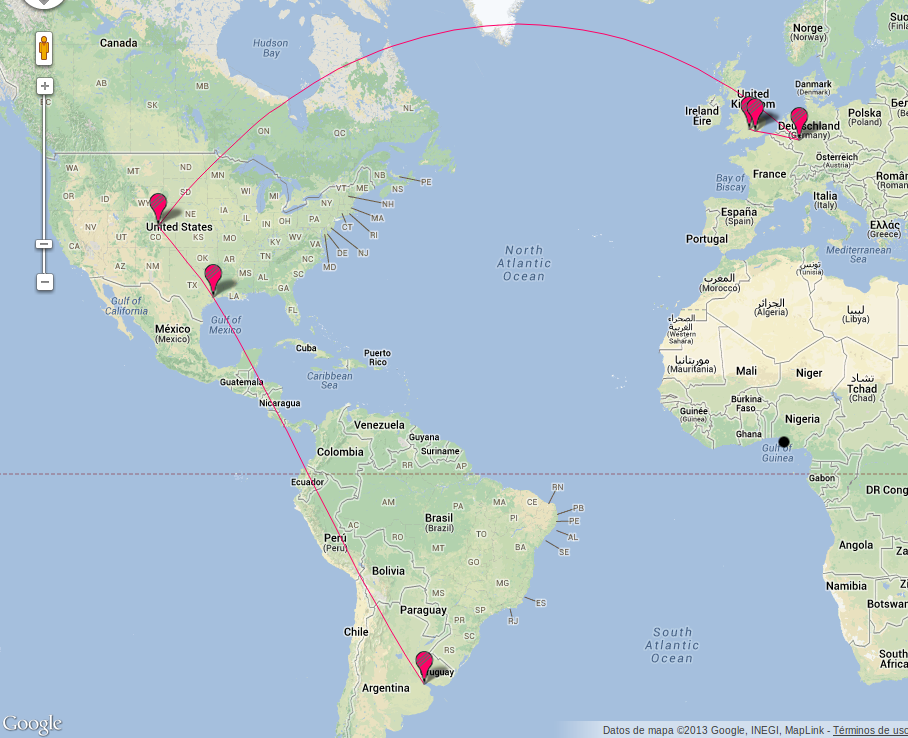
\includegraphics[width=0.9\textwidth]{imgs/inglaterra_ruta_1.png}
    \caption{Mapa con la ruta aproximada hacia el host \url{www.ox.ac.uk} (Reino Unido)}
    \label{fig:ruta_ing}
\end{figure}

\begin{figure}[H]
  \centering
    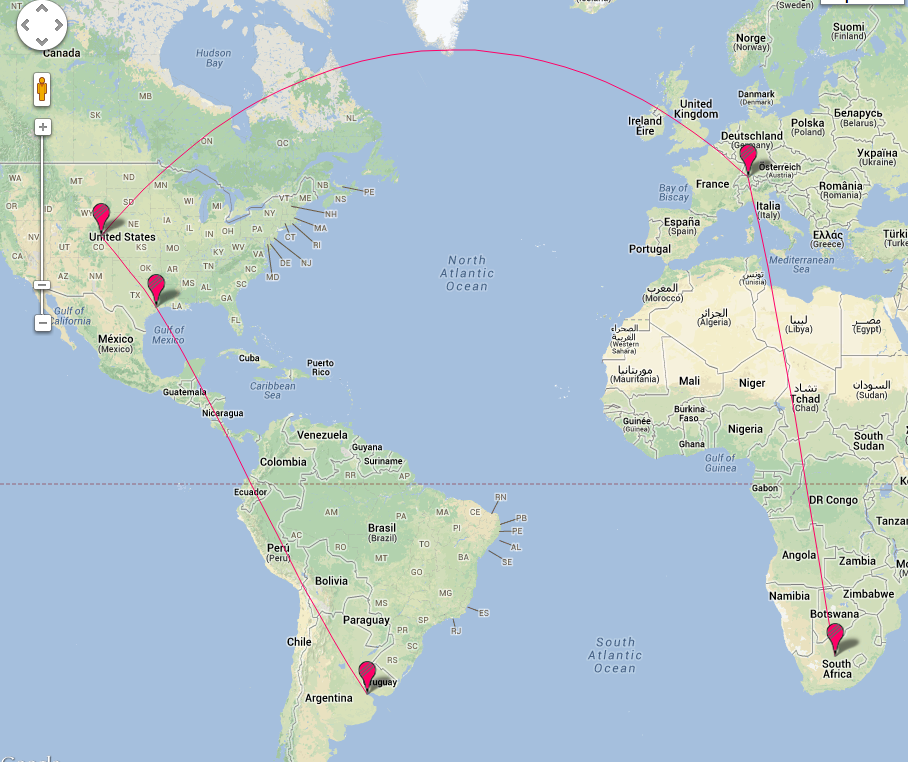
\includegraphics[width=0.9\textwidth]{imgs/sudafrica_ruta_1.png}
    \caption{Mapa con la ruta aproximada hacia el host \url{web.up.ac.za} (Sud\'africa)}
    \label{fig:ruta_sud}
\end{figure}

La figura \ref{fig:ruta_sud} es un ejemplo de cuan ineficiente puede ser el camino hacia el destino. En este caso es probable que se deba a la falta de enlaces directos entre América y Africa.\\

Es interesante tambi\'en observar c\'omo var\'ia el RTT medido seg\'un distintos momentos del d\'ia.

\begin{figure}[H]
  \centering
    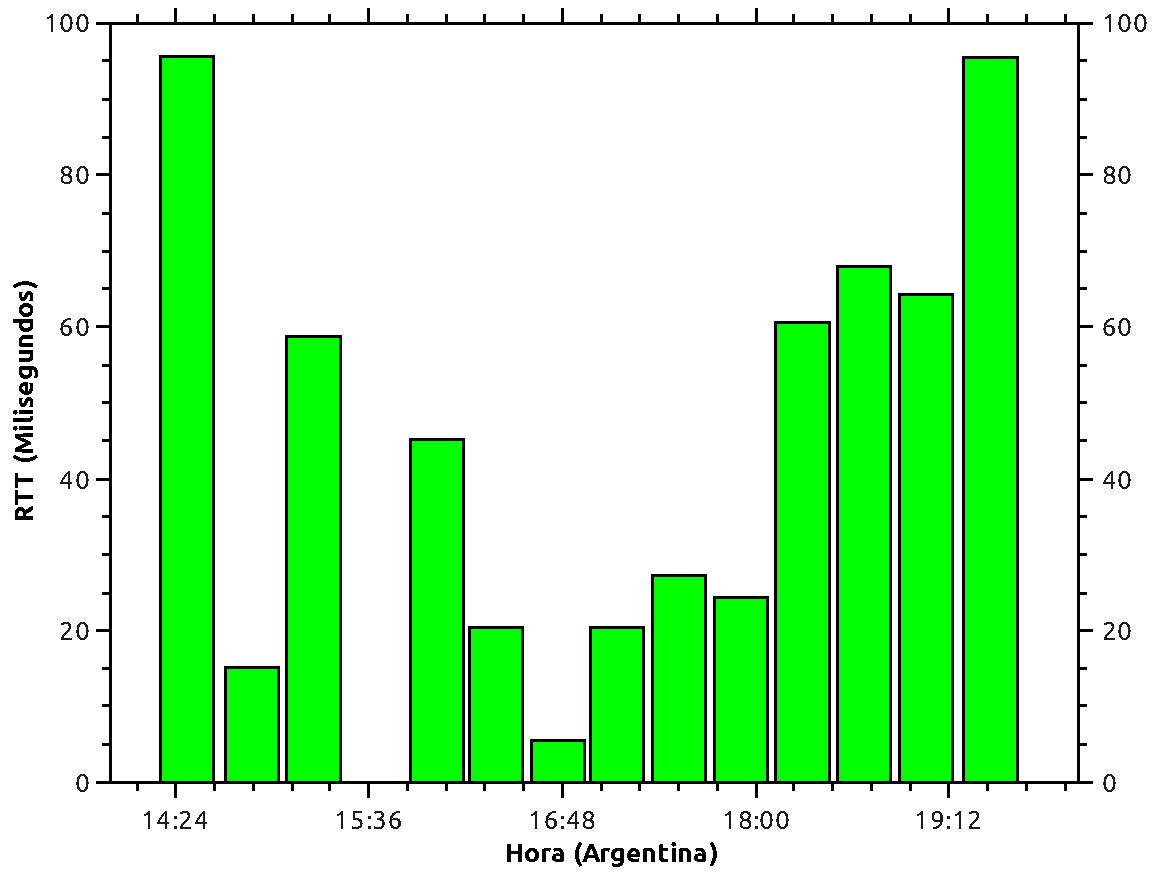
\includegraphics[width=0.8\textwidth]{graficos/rtts_dia_finlandia.pdf}
    \caption{RTTs medidos a lo largo del dia en el enlace EEUU-Inglaterra}
    \label{fig:rtts_fin}
\end{figure}

\begin{figure}[H]
  \centering
    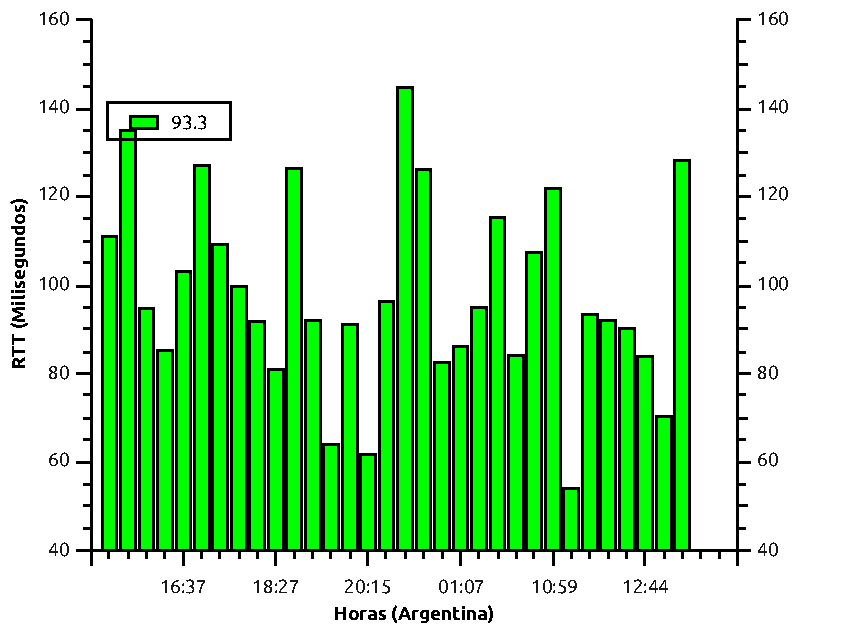
\includegraphics[width=0.8\textwidth]{graficos/rtts_dia_inglaterra.pdf}
    \caption{RTTs medidos a lo largo del dia en el enlace EEUU-Alemania}
    \label{fig:rtts_ing}
\end{figure}

\begin{figure}[H]
  \centering
    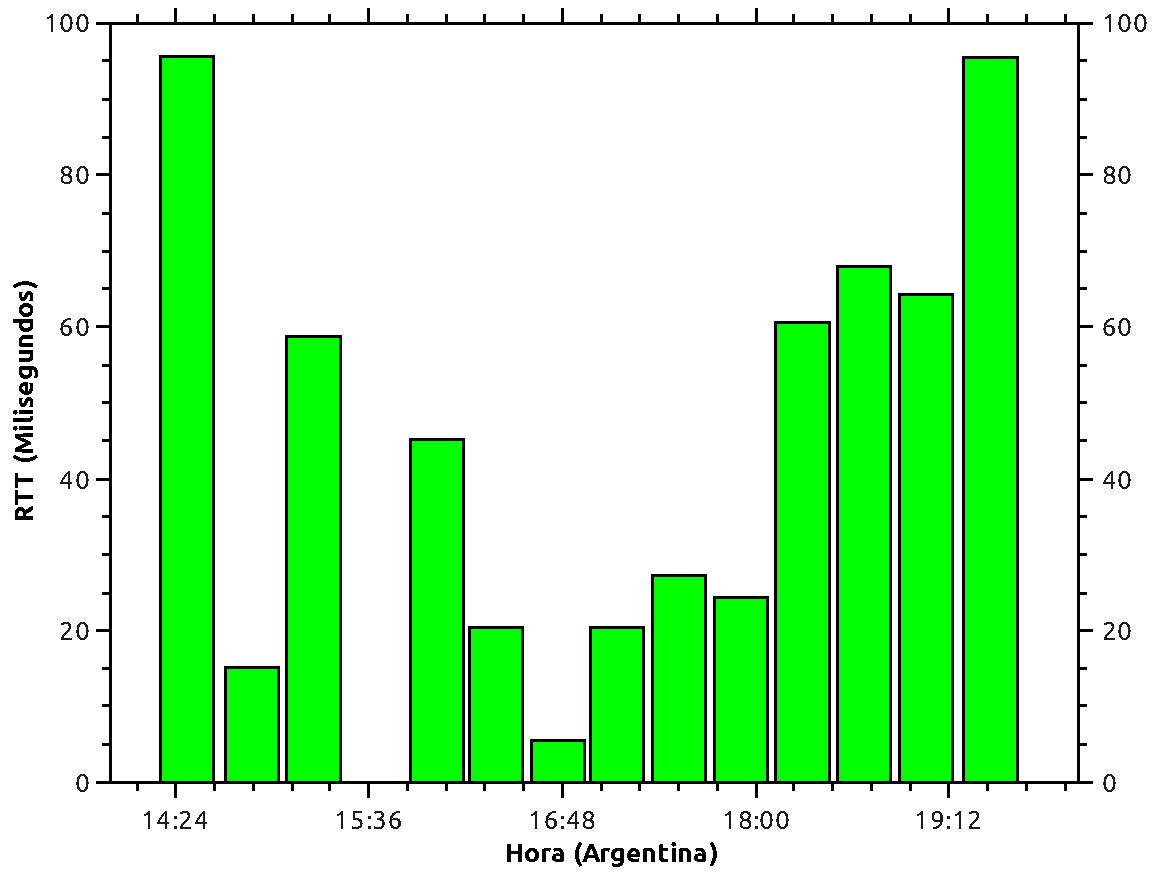
\includegraphics[width=0.8\textwidth]{graficos/rtts_dia_finlandia.pdf}
    \caption{RTTs medidos a lo largo del dia en el enlace EEUU-Suiza}
    \label{fig:rtts_sud}
\end{figure}

%EEUU : -3
%FINLANDIA: +4
En las figura \ref{fig:rtts_fin}, \ref{fig:rtts_ing} y \ref{fig:rtts_sud} se puede ver cómo los RTT varían constantemente durante todo el día, mostrando picos a ciertas horas. Estos enlaces no sólo son utilizados por Estados Unidos, sino también por varios hosts ubicados en todo el continente americano. De hecho, los tres enlaces encontrados tienen en una de sus puntas Estados Unidos, Colorado, lo cual pareciera indicar que es un punto de alto tráfico. Debido a las diferencias horarias entre ambos continente, es factible que mientras en algunos países el tráfico es muy intenso, en otros no sea esperable que se congestione la red, por lo cual no se puede predecir cual va a ser la hora de más alto tráfico. \\

Al comparar los valores medidos de RTT con el calculado (tabla \ref{tabla1}) nos encontramos con que el valor calculado no es correcto, ya que en muchos casos se obtienen RTTs menores a este. Atribuimos esto a la inestabilidad de nuestro método de medición y la dificultad de determinar efectivamente la ubicación de los extremos del enlace. En las mediciones aparecieron incluso RTTs ``negativos'': casos en los que el RTT del paquete envíado hacia Europa era menor que el envíado hacia América. Estos errores tienen que ver también con el método utilizado para hacer el traceroute: puede ser que al enviar el mensaje hacia Estados Unidos haya mucha congestión, mientras que al paso siguiente, al enviar hacia Europa, este problema ya se encuentre solucionado, con lo cual el tiempo es menor. Los RTTs negativos se observan incluso al tomar promedio, si bien hacer esto permite suavizar bastante las diferencias entre cada envío de paquete.\\

%De todas formas, pese a esto se pueden ver a grandes rasgos cómo a las 16hs de Argentina, el cual equivale a un rango de entre las 11hs y las 16hs de todo el continente americano, este enlace parece estar mucho menos congestionado que entre las 16 y las 20hs. 

%%% Aca hay q pulirlo.. esta medio chori.. le falta poder de sintesis :P, capas meter alguna tabla con zonas horarias.. y sacar alguna conclusion de trafico segun momento del dia..

En el caso de la figura \ref{fig:rtts_ing} se puede ver que, si bien se observan picos en los horarios laborables, durante el resto del día no existe una tendencia o valor representativo. Este es un ejemplo de lo caótico e irregular que puede llegar a ser el tráfico en Internet. Con respecto al RTT mínimo calculado, en este caso observamos que todas las mediciones están por arriba de él, algunas de ellas considerablemente, lo cual era lo esperable. Más allá de la inestabilidad manifestada anteriormente, aquí podemos ver que la mayoría de las mediciones resultan entre $80$ms y $100$ms, lo que evidencia que, para comunicaciones de realmente larga distancia, el factor geográfico sigue siendo el mayor limitante en cuanto a la demora promedio (por sobre los tiempos de demora de funcionamiento del protocolo en sí, como por ejemplo, las colas de los routers y las decisiones de routeo).\\

Por último, experimentamos el uso de los enlaces encontrados a través del envío de sondas de traceroute hacia otras páginas de la zona. Los enlaces encontrados para cada uno de los casos fueron los siguientes:

\begin{center}
\begin{tabular}{l l l}
  \textbf{País Destino} & \textbf{url} & \textbf{Enlace} \\
  \hline \\
 \textbf{Suecia} & www.gu.se & Entre 67.16.139.18 y 213.155.137.30\\
  & www.lunduniversity.lu.se & Entre 67.16.139.18 y 213.155.137.26\\
  \textbf{Finlandia} & www.uta.fi & Entre 67.16.139.18 y 213.155.137.26\\
    & www.utu.fi & Entre 67.16.139.18 y 213.155.137.26\\
   \textbf{Inglaterra} & www.buckingham.ac.uk & Entre 67.16.139.18 y 213.200.84.37\\
    & www.city.ac.uk & Entre 67.16.139.18 y 141.136.107.41\\
    \textbf{Escocia} & www.dundee.ac.uk & Entre 67.16.139.18 y 141.136.109.158\\
     & www.stir.ac.uk & Entre 67.16.139.18 y 141.136.109.158\\
     \textbf{Sudáfrica} & www.ul.ac.za & 146.82.32.154 y 77.109.128.149\\
      & www.ukzn.ac.za & 146.82.32.154 y 77.109.128.149\\
       & www.nmmu.ac.za & 146.82.32.154 y 77.109.128.146\\
        & www.unisa.ac.za & 146.82.32.154 y 77.109.128.149
 \end{tabular}
 \end{center}
 
 
 Si bien en algunos casos varía la ip del enlace original, en todas estas pruebas la localización del enlace sigue siendo la misma, lo cual indica que el enlace encontrado es utilizado dentro de la zona. Con respecto a la ruta tomada, tampoco se observan muchas diferencias. Si bien pueden aparecer nodos que en la ruta hacia los hosts originales no aparecían, la ruta tomada en general (la que se observa en las figuras \ref{fig:ruta_fin}, \ref{fig:ruta_ing} y \ref{fig:ruta_sud}) se observa en todos los casos. 


$\\$	
\section{Conclusiones}



%\newpage
%\begin{thebibliography}{9}
 %\end{thebibliography}


\end{document}

